% Portfolio website — technical architecture (single-page overview)
% Build: pdflatex web-architecture.tex (twice if references/hyperref complain)

\documentclass[10pt,a4paper]{article}
\usepackage[utf8]{inputenc}
\usepackage[T1]{fontenc}
\usepackage[margin=1.35cm]{geometry}
\usepackage{microtype}
\usepackage{booktabs}
\usepackage{enumitem}
\usepackage{tikz}
\usetikzlibrary{positioning,arrows.meta,fit,calc}

\setlist{nosep,leftmargin=*}
\setlength{\parskip}{0.35em}
\setlength{\parindent}{0pt}
\usepackage[hidelinks]{hyperref}

\title{\textbf{Technical Architecture}\\[0.25em]\large Student portfolio website (web development assignment)}
\author{\textbf{Mamekem Rosly}\\[0.35em]\normalsize African Institute for Mathematical Sciences (AIMS) --- Senegal\\\small\textit{Master's student --- Applied Mathematics (Computer Security \& Machine Learning)}}
\date{\today}

\begin{document}
\maketitle
\vspace{-1.8em}

\begin{center}
\fbox{\parbox{0.94\linewidth}{\centering\footnotesize
\textbf{AIMS assignment context.} Student-authored portfolio for a web-development coursework component; this one-pager documents the technical architecture of that deliverable.}}
\end{center}
\vspace{0.25em}

\begin{center}
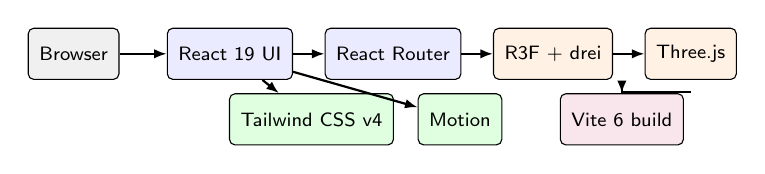
\begin{tikzpicture}[
  font=\scriptsize\sffamily,
  box/.style={draw, rounded corners=2pt, minimum height=6.5mm, inner xsep=4pt, inner ysep=2pt},
  arr/.style={-{Latex[length=1.6mm]}, thick},
]
  \node[box, fill=gray!12] (ua) {Browser};
  \node[box, fill=blue!8, right=6mm of ua] (react) {React 19 UI};
  \node[box, fill=blue!8, right=4mm of react] (rr) {React Router};
  \node[box, fill=orange!10, right=4mm of rr] (r3f) {R3F + drei};
  \node[box, fill=orange!10, right=4mm of r3f] (three) {Three.js};
  \node[box, fill=green!12, below=5mm of $(react)!0.5!(rr)$] (tw) {Tailwind CSS v4};
  \node[box, fill=green!12, right=3mm of tw] (motion) {Motion};
  \node[box, fill=purple!10, below=5mm of $(r3f)!0.5!(three)$] (vite) {Vite 6 build};
  \draw[arr] (ua) -- (react);
  \draw[arr] (react) -- (rr);
  \draw[arr] (rr) -- (r3f);
  \draw[arr] (r3f) -- (three);
  \draw[arr] (react) -- (tw);
  \draw[arr] (react) -- (motion);
  \draw[arr] (three.south) ++(0,-0.15) -| (vite.north);
\end{tikzpicture}
\end{center}

\vspace{0.3em}
\textbf{Purpose.} As an AIMS student, I implemented this portfolio to showcase research interests, projects, and credentials. The site is a client-side rendered (CSR) single-page application (SPA) with one extra route for a certifications gallery. Content is authored in TypeScript/React; styling is utility-first; the hero and project sections embed interactive 3D scenes for engagement and demonstration of modern front-end skills.

\textbf{Presentation layer.} \textsf{React~19} and \textsf{TypeScript} structure the UI into pages (\texttt{App.tsx}, \texttt{pages/Certifications.tsx}) and components (\texttt{Scene}, \texttt{ProjectCarousel}, \texttt{CipherGate}, etc.). \textsf{Tailwind CSS~v4} (via \texttt{@tailwindcss/vite}) supplies design tokens and responsive layout. \textsf{Motion} drives scroll/viewport animations. \textsf{lucide-react} provides icons.

\textbf{Navigation \& state.} \textsf{react-router-dom} maps paths (\texttt{/}, \texttt{/certifications}). Local UI state uses React hooks. Theme (\texttt{ThemeContext}) toggles light/dark, persists \texttt{portfolio-theme} in \texttt{localStorage}, mirrors \texttt{html.light} for global CSS overrides, and feeds accent colors into Three.js materials where needed.

\textbf{3D \& media.} \textsf{@react-three/fiber} bridges React to \textsf{Three.js}: background particle field (\texttt{Scene}), carousel project cards with textures (\texttt{ProjectCarousel}), lighting and fog. \textsf{@react-three/drei} adds helpers (\texttt{Image}, \texttt{Text}, \texttt{Grid}, etc.). Raster assets ship as bundled imports (Vite).

\textbf{Build \& delivery.} \textsf{Vite~6} with \texttt{@vitejs/plugin-react} bundles ESM for production (\texttt{npm run build} $\rightarrow$ \texttt{dist/}). Typical deployment is static hosting (e.g.\ Vercel).

\textbf{Security / UX extras.} A gated section (\texttt{CipherGate}) conditionally reveals content after a client-side puzzle. No server is required for the static portfolio shell; optional Node packages in the repo may support separate tooling and are not part of the static export unless explicitly wired.

\vspace{0.25em}
\begin{table}[h]
  \centering
  \scriptsize
  \begin{tabular}{@{}ll@{}}
    \toprule
    \textbf{Concern} & \textbf{Primary technologies} \\
    \midrule
    UI framework & React 19, TypeScript \\
    Styling & Tailwind CSS 4 (\texttt{@tailwindcss/vite}) \\
    Routing & react-router-dom 7 \\
    Animation & Motion 12 \\
    3D & three, @react-three/fiber 9, @react-three/drei 10 \\
    Tooling & Vite 6, ESLint-style check via \texttt{tsc --noEmit} \\
    \bottomrule
  \end{tabular}
\end{table}

\end{document}
